\documentclass{article}
\usepackage{graphicx} % Required for inserting images
\usepackage[utf8]{inputenc}
\usepackage{amsmath}
\usepackage[margin=1in]{geometry}

\title{\huge Topical note on Numerical Method lecture 1}
\author{Prepared by Debashish Chakraborty \\
Based on lecture by Professor Kazi Ashrafuzzaman \\
MAT-431}
\date{22.5.2025}

\begin{document}

\maketitle
Numerical Method's alternative name is Scientific Computing. 

\section{Normal Distribution CDF}
Normal distributions's PDF cannot be integrated in closed form.
\begin{figure}[htbp]
  \centering
  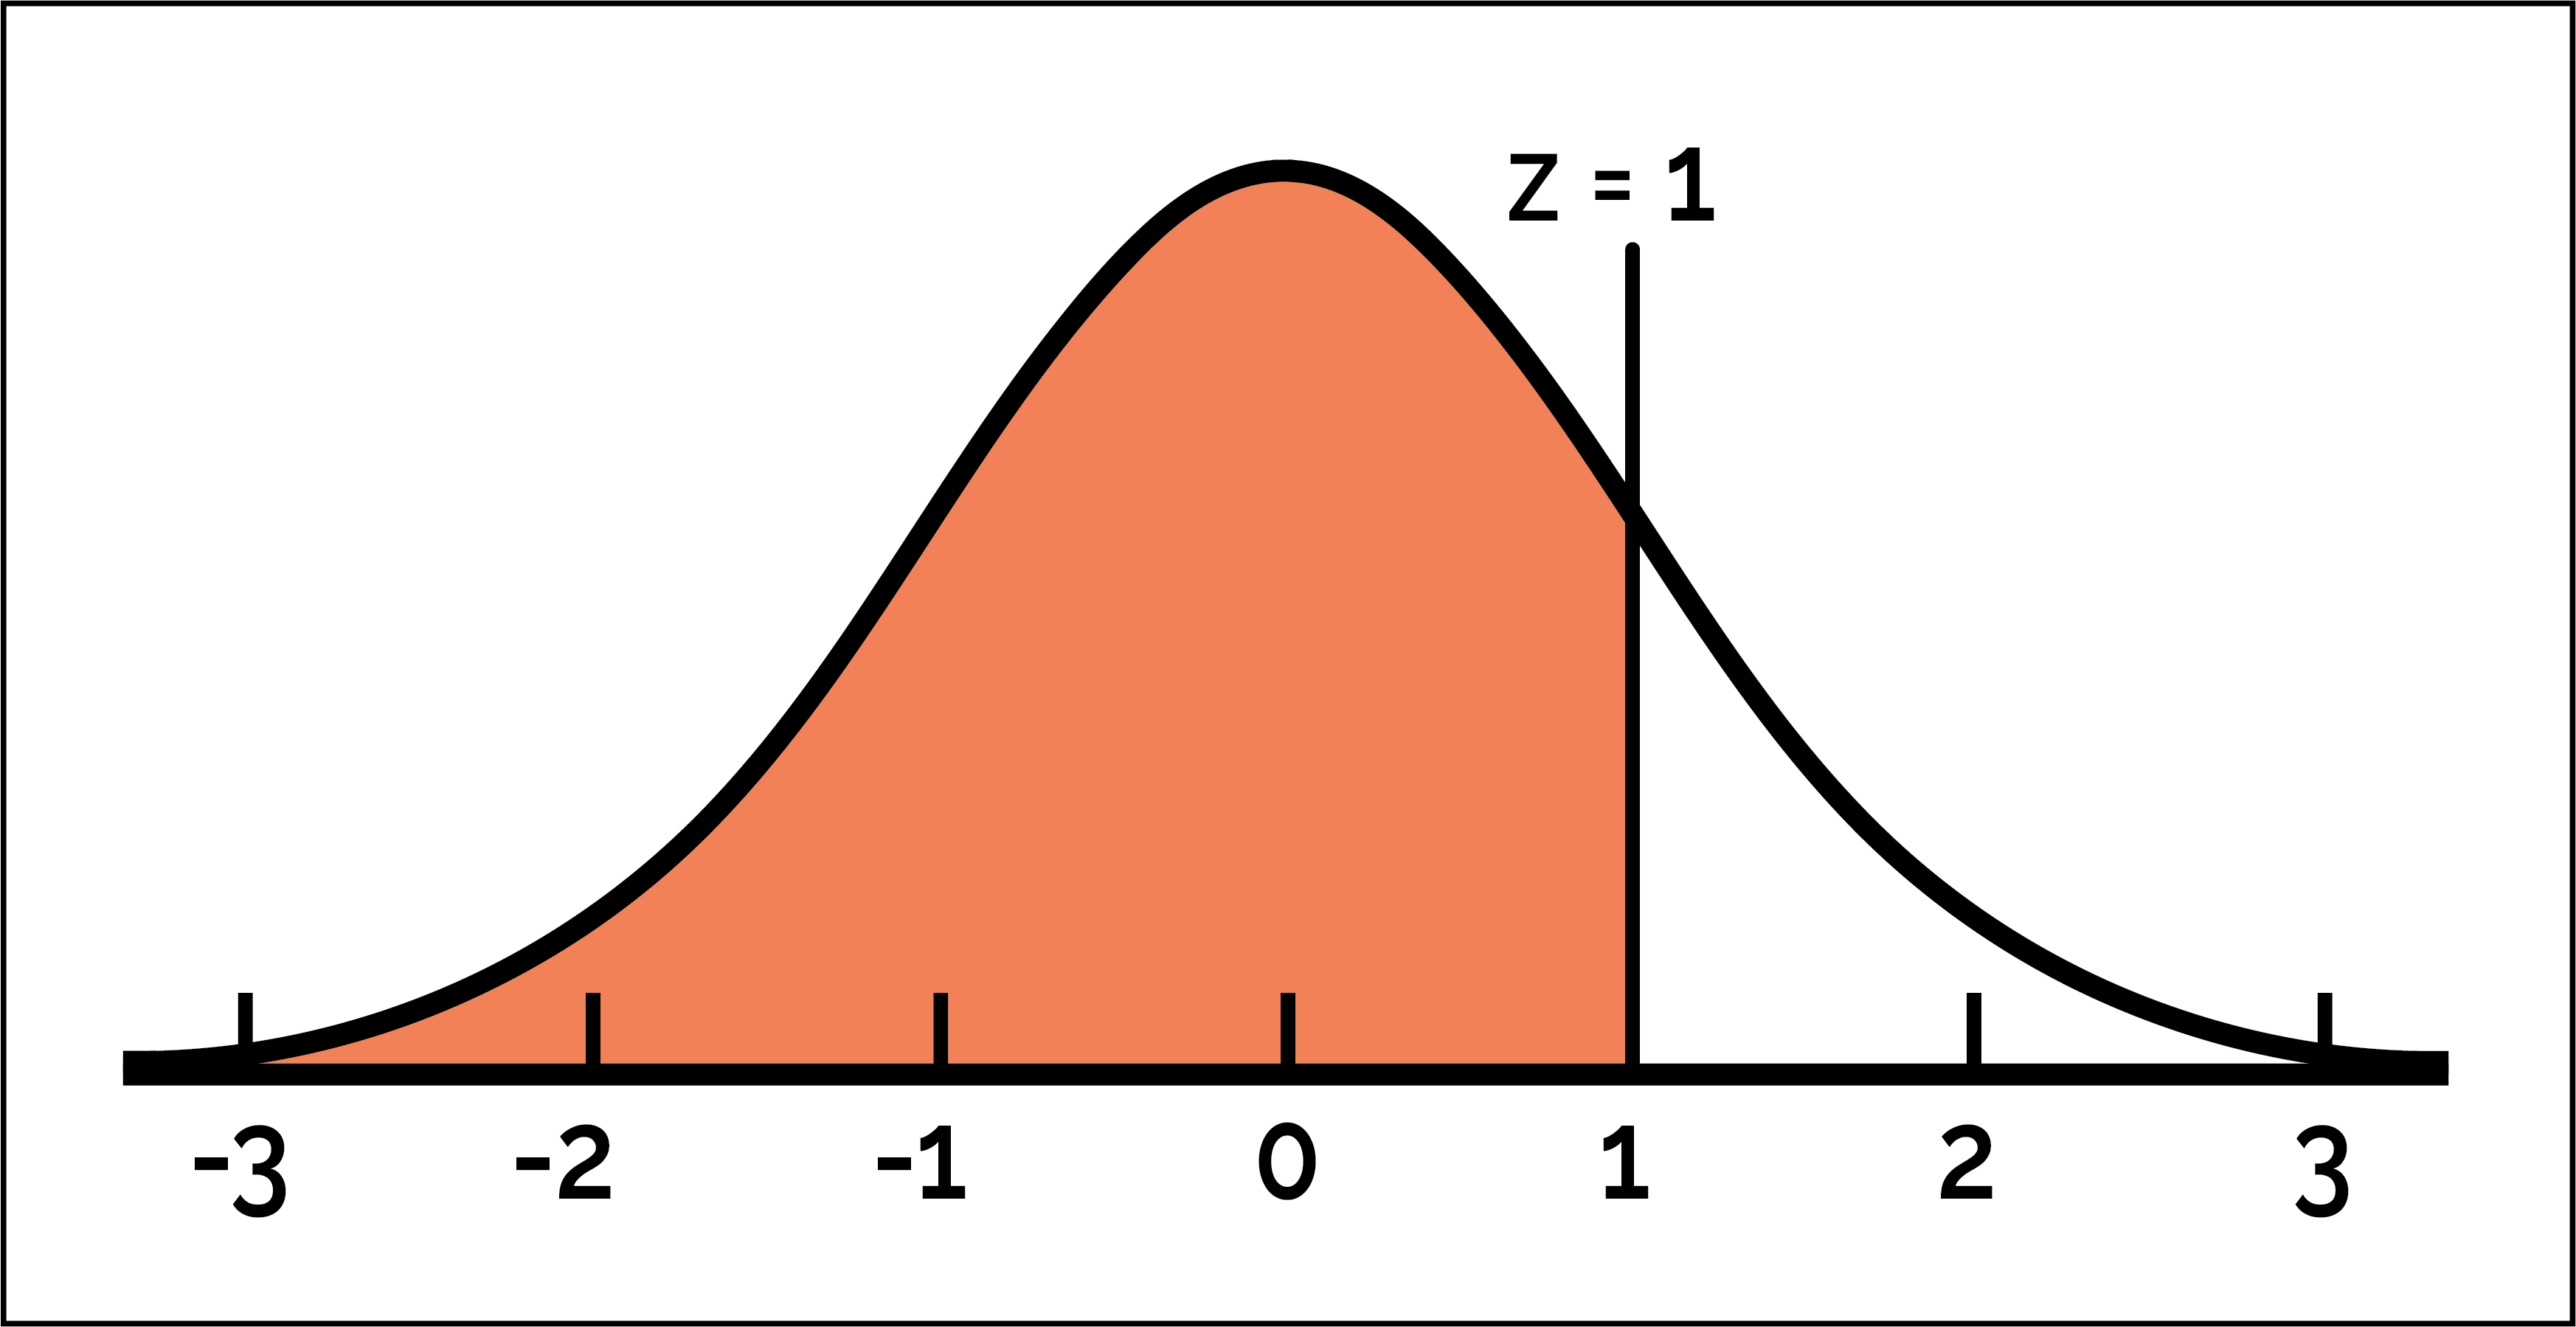
\includegraphics[width=0.6\textwidth]{Normal_Distribution.png}
\end{figure}


Normal Distribution CDF, 
$$f_X(x) = \int_{-\infty}^x \frac{1}{\sqrt{2\pi}}e^{-\frac{y^2}{2}}dy$$

We can compute this integral using various methods. \\
\begin{enumerate}
\item \textbf{Riemann Sum:} A Riemann sum approximates the definite integral of a function by summing the areas of rectangles under the curve

\item \textbf{Monte Carlo Method:} The Monte Carlo method for computing integrals approximates the value of a definite integral by using random sampling and averaging.

\item \textbf{Quadratic Equation:} Using random 3 points we can get a quadratic equation from which we can calculate the area more accurately.

\end{enumerate}

\textbf{Lab assignment 1:}  Write a program to calculate the normal distribution CDF using random points(Monte-Carlo method).
\newpage
\section{Modeling}
In the realm of numerical methods, "modeling" refers to creating a mathematical representation of a real world physical system or phenomenon to predict its behavior. 
\begin{itemize}
    \item \textbf{Approximation: } Approximation in modeling refers to the practice of using simplified representations or techniques to analyze complex systems, while acknowledging that the model is not a perfect replica of the real-world situation.

    \item \textbf{Modeling Errors: }
    \begin{enumerate}
\item Formatting Error

\item Quantization Error

\item Rounding Error

\item Absolute Error

\item Relative Error

\end{enumerate}
    
\end{itemize}

\section{Catastrophic Cancellation:}
When we substract a very small number(electron mass) from a very big number like Avogadro's number($6.023 * 10^{23}$), the result seems to be the big number and the smaller number is completely ignored, this phenomenon is called catastropic cancellation.

\section{Floating point sum}
We can compute the floating point sum using 3 methods.
\begin{enumerate}
\item Random sum

\item Increasing sum

\item Decreasing sum

\end{enumerate}
\textbf{Lab assignment 2:} Write a program to calculate the sum of 10000 floating point numbers.

\section{Linear and Non-linear equation}
\subsection{Linear Equation:}
$f(x)$ is linear iff for scalars $a$ and $b$ with points $x_1$ and $x_2$,
$$f(ax_1 + bx_2) = af(x_1) + bf(x_2)$$
\subsection{Non-Linear Equation:} 
\begin{enumerate}
\item  \textbf{Transcendental equation:} A transcendental nonlinear equation is an equation involving functions that are not algebraic, meaning they cannot be expressed as a solution to a polynomial equation. Examples include equations involving trigonometric, logarithmic, or exponential functions. 

\item \textbf{Algebraic equation:} An equation of the type $f(x) = 0$ is algebraic if it contains power of $x$, that is, $f(x)$ is a polynomial.


\end{enumerate}
\newpage 
\section{Analytical Question}

\subsection{}
\begin{figure}[htbp]
  \centering
  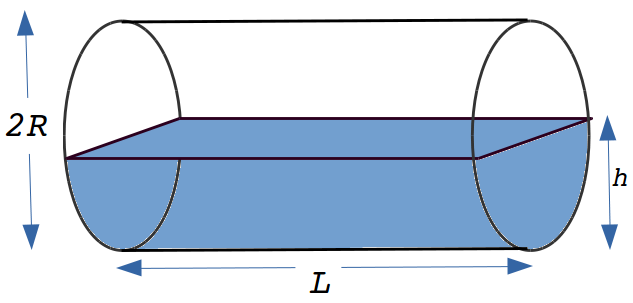
\includegraphics[width=0.6\textwidth]{cylinder.png} % change filename and size as needed
  
  \label{fig:my_label}
\end{figure}
A cylinder is lying on the horizontal side and it is continuously filling with water through a pipe. What would be the height($h$) of the water level from the ground to fill up quarter($\frac{1}{4}$) of the volume of that cylinder?

\subsection{}
Represent the fibonacci number recurrence using 2*2 matrices.

\end{document}
